\documentclass[11pt,a4paper]{article}

% ---------------------------------------------------------------- packages
\usepackage[T1]{fontenc}
\usepackage{newtxtext,newtxmath}
\usepackage[a4paper,margin=2.3cm,headheight=14pt]{geometry}
\usepackage{fancyhdr}
\usepackage{lastpage}
\usepackage{needspace}
\usepackage{graphicx}
\usepackage{float}
\usepackage{booktabs}
\usepackage{tabularx}
\usepackage{array}
\usepackage[table]{xcolor}
\usepackage{amsmath}
\usepackage{enumitem}
\usepackage[font=small,labelfont=bf]{caption}
\usepackage{subcaption}
\usepackage{titlesec}
\usepackage[hidelinks]{hyperref}

\graphicspath{{figures/}}
\setlength{\parindent}{1.5em}
\setlength{\parskip}{3pt}
\linespread{1.08}
\renewcommand{\arraystretch}{1.18}
\definecolor{navy}{HTML}{1F3A5F}
\definecolor{lightrow}{HTML}{EEF2F7}
\definecolor{bestrow}{HTML}{F6E3DF}
\newcolumntype{Y}{>{\raggedright\arraybackslash}X}

\titleformat{\section}{\Large\bfseries}{\thesection.}{0.6em}{}
\titleformat{\subsection}{\large\bfseries}{\thesubsection.}{0.6em}{}
\titlespacing*{\section}{0pt}{14pt}{6pt}
\titlespacing*{\subsection}{0pt}{10pt}{4pt}

\pagestyle{fancy}
\fancyhf{}
\fancyhead[L]{\small MACHINE LEARNING \textbar{} PBL REPORT}
\fancyhead[R]{\small UNIVERSITY OF RWANDA}
\fancyfoot[C]{\small \thepage\ / \pageref{LastPage}}
\renewcommand{\headrulewidth}{0.5pt}

\setlist[itemize]{leftmargin=1.6em,itemsep=2pt,topsep=3pt}
\setlist[enumerate]{leftmargin=1.8em,itemsep=2pt,topsep=3pt}

\hypersetup{pdftitle={Predicting Unemployment among Rwandan Youth with Machine Learning},
            pdfauthor={Niyobyose Brancal}}

\begin{document}

% ================================================================= COVER
\begin{titlepage}
\centering
\vspace*{1.5cm}
{\Large\bfseries UNIVERSITY OF RWANDA\par}
\vspace{0.3cm}
{\large COLLEGE OF SCIENCE AND TECHNOLOGY\par}
{SCHOOL OF SCIENCE\par}
{DEPARTMENT OF MATHEMATICS\par}
\vspace{2cm}
\rule{0.85\textwidth}{1pt}\par\vspace{0.3cm}
{MACHINE LEARNING: PROJECT-BASED LEARNING (PBL) REPORT\par}
\vspace{0.6cm}
{\LARGE\bfseries Predicting Unemployment among Rwandan Youth\\[4pt]
with Machine Learning: Evidence from the\\[4pt] 2025 Labour Force Survey\par}
\vspace{0.4cm}
\rule{0.85\textwidth}{1pt}\par
\vspace{2cm}
\begin{tabular}{@{}p{5cm}p{7cm}@{}}
\textbf{Student name}        & Niyobyose Brancal \\
\textbf{Registration number} & 223014431 \\
\textbf{Department}          & Mathematics \\
\textbf{Programme}           & Statistics \\
\textbf{Course}              & Machine Learning \\
\textbf{Lecturer}            & Prof.\ Nzabanita Joseph \\
\textbf{Software}            & R (caret, ranger, gbm, pROC, Shiny)
\end{tabular}
\vfill
{Kigali, Rwanda\par}
{November 2026\par}
\end{titlepage}
\setcounter{page}{2}

% ================================================================= ABSTRACT
\section*{Abstract}
\addcontentsline{toc}{section}{Abstract}
Youth unemployment is one of Rwanda's main social and economic challenges. This project uses the
2025 Rwanda Labour Force Survey (LFS) to build machine-learning models that classify young people
aged 16--30 who are in the labour force as \emph{employed} or \emph{unemployed}. After cleaning, the
analysis sample contains 15{,}958 youth, of whom 14.7\% are unemployed, so the two classes are
strongly imbalanced. Seventeen demographic, educational, geographic and household predictors were
used. Ten algorithms were trained in R with the \texttt{caret} package: logistic regression, Lasso,
elastic net, linear and regularized discriminant analysis (LDA, RDA), naive Bayes, $k$-nearest
neighbours (KNN), a decision tree, random forest and gradient boosting (GBM). The data were split
70/30 into training and test sets, hyper-parameters were tuned with 5-fold cross-validation, and the
training folds were down-sampled to balance the classes. Models were compared with ROC AUC, recall,
specificity, precision, $F_1$ and Cohen's $\kappa$.

The random forest achieved the highest test ROC AUC (0.676; 95\% CI 0.656--0.696) and found 62\% of
unemployed youth at the default cut-off, although its advantage over GBM, LDA and Lasso was not
statistically significant (DeLong test). The most informative factors were district, position in the
household, age, years of schooling and household size. The results confirm an \emph{education
paradox}: youth with upper secondary or university education face a higher risk of unemployment than
youth with little schooling. Young women and youth who are not household heads are also more at
risk. Predictive power is modest, showing that unemployment depends on many factors the survey does
not measure. A Shiny web application was developed to share the results and offer an interactive
risk calculator.

\medskip\noindent\textbf{Keywords:} youth unemployment; Rwanda; Labour Force Survey; classification;
random forest; imbalanced data; ROC AUC.

\newpage
\tableofcontents
\newpage

% ================================================================= 1
\section{Problem Identification and Translation}

\subsection{Background}
Rwanda's policies on skills development, job creation and economic transformation depend on reliable
knowledge of who has access to work. Every year many young people complete school or vocational
training and look for their first job. According to the National Institute of Statistics of Rwanda
(NISR), the unemployment rate among persons aged 16--30 was \textbf{15.7\%} in May 2026 and
\textbf{18.8\%} in August 2026, compared with 11.9\% and 13.1\% for adults aged 31 and above
\cite{nisr_q2,nisr_q3}. Young people are therefore clearly more affected than older workers.

Having a job is not the end of the story either: in 2024 about 90.4\% of total employment in Rwanda
was informal \cite{nisr_annual}, and the World Bank reports that more than one million young
Rwandans were neither in employment, education nor training in 2024 \cite{worldbank}. Earlier
studies in Rwanda found that gender, age, education and location are associated with youth
employment \cite{ndagijimana,afdb}. Human capital theory predicts that more education should improve
job chances \cite{becker,mincer}, while job-search and matching theories explain why educated youth
may remain unemployed longer while they wait for suitable work. Knowing \emph{who} is most at risk
helps government and training institutions to target employment services, career guidance and
work-based learning.

\subsection{Problem statement}
Headline unemployment rates show how many young people are unemployed, but not which individual
characteristics most strongly predict unemployment, nor how well these characteristics can identify
an at-risk young person. This project translates the social problem into a \textbf{supervised binary
classification problem}:

\begin{quote}
\itshape Given the demographic, educational, geographic and household characteristics of a young
person aged 16--30 who is in the labour force, predict whether the person is Employed or Unemployed.
\end{quote}

\noindent Formally, for youth $i$ with predictor vector $\mathbf{x}_i$, the target is
\begin{equation}
Y_i=\begin{cases}1 & \text{if the young person is unemployed (positive class)},\\
0 & \text{if the young person is employed,}\end{cases}
\end{equation}
and each model estimates a risk score $\hat p(\mathbf{x}_i)=\widehat{P}(Y_i=1\mid\mathbf{x}_i)$. A
young person is classified as unemployed when $\hat p(\mathbf{x}_i)\ge c$, with default cut-off
$c=0.5$. The target is the official NISR labour-force status \cite{ilo}. Youth outside the labour
force (mainly full-time students) are not part of this task.

\subsection{Research gap and objectives}
The author's research-methodology proposal studies the factors \emph{associated} with labour-force
status using survey-weighted statistics. Existing Rwandan studies \cite{ndagijimana,afdb} relied on
older survey designs and classical regression. There is little evidence on how well modern
machine-learning methods can \emph{predict} individual unemployment risk with the redesigned LFS, or
on which method works best. This project fills that gap with a predictive approach.

\medskip\noindent\textbf{General objective.} To build, compare and interpret machine-learning models
that predict unemployment among Rwandan youth (16--30) in the labour force, using the 2025 LFS.

\needspace{6\baselineskip}\medskip\noindent\textbf{Specific objectives.}
\begin{enumerate}
\item To prepare a clean, leakage-free modelling dataset from the 2025 LFS microdata and describe it.
\item To train and tune at least eight classification algorithms using 5-fold cross-validation.
\item To compare the models on an unseen test set (30\% of the data) with ROC AUC as the main metric,
      together with recall, specificity, precision, $F_1$ and $\kappa$, and to test whether the
      differences are statistically significant.
\item To identify the factors that most strongly predict youth unemployment and the direction of
      their effects.
\item To evaluate how well the best model performs for women, men, urban and rural youth.
\item To communicate the findings through an interactive web application (bonus task).
\end{enumerate}

% ================================================================= 2
\section{Machine Learning Methodology}

\subsection{Data source and description}
The data come from the \textbf{Rwanda Labour Force Survey 2025}, an official open-access survey
conducted by NISR and distributed through its microdata catalogue \cite{nisr_micro25}. The LFS is a
nationally representative household survey based on a stratified two-stage design: enumeration areas
are selected with probability proportional to size, and households are then selected within each
area. Trained enumerators interview household members face to face each quarter, and households are
revisited in a rotating panel \cite{nisr_method}. Labour-force status follows the international ILO
definitions \cite{ilo} and variable names follow the NISR data dictionary \cite{nisr_dict}. The raw
file contains \textbf{100{,}852 person records and 207 variables}. Table~\ref{tab:flow} summarises
how the modelling dataset was obtained and Table~\ref{tab:vars} describes its variables.

\begin{table}[H]
\centering
\caption{From the raw survey file to the modelling dataset}
\label{tab:flow}
\rowcolors{2}{lightrow}{white}
\begin{tabularx}{\textwidth}{@{}l r Y@{}}
\toprule
\textbf{Step} & \textbf{Records} & \textbf{Comment} \\
\midrule
Raw LFS 2025 file & 100{,}852 & All persons interviewed, 207 variables \\
Youth aged 16--30 & 26{,}290 & NISR youth definition \\
Exact duplicates removed & 26{,}289 & 1 identical record \\
Keep youth in the labour force & 15{,}960 & 10{,}329 youth outside the labour force excluded \\
Remove missing years of schooling & 15{,}958 & 2 records \\
\textbf{Final modelling dataset} & \textbf{15{,}958} & \textbf{13{,}605 employed (85.3\%); 2{,}353 unemployed (14.7\%)} \\
\bottomrule
\end{tabularx}
\end{table}

\begin{table}[H]
\centering
\caption{Variables in the modelling dataset (one target and 17 predictors)}
\label{tab:vars}
\small
\rowcolors{2}{lightrow}{white}
\begin{tabularx}{\textwidth}{@{}l l Y@{}}
\toprule
\textbf{Variable} & \textbf{Type} & \textbf{Values / levels} \\
\midrule
Employment status (target) & Binary & Employed, Unemployed \\
Age & Numeric & 16--30 years \\
Sex & Categorical (2) & Male, Female \\
Education level & Categorical (5) & None, Primary, Lower secondary, Upper secondary, University \\
Years of schooling & Numeric & 0--21 years \\
Currently a student & Categorical (2) & Yes, No \\
Residence & Categorical (2) & Urban, Rural \\
District & Categorical (30) & All 30 districts of Rwanda \\
Marital status & Categorical (4) & Married, Living together, Previously married, Single \\
TVET training & Categorical (3) & Yes, No, Not stated \\
Disability & Categorical (2) & Yes, No \\
Household size & Numeric & 1--10 (10 means ten or more) \\
Relationship to household head & Categorical (9) & Head, spouse, child, sibling, grandchild, other relative, domestic worker, non-relative, other \\
Field of education & Categorical (10) & General, education, humanities, social science, science, engineering, agriculture, health, services, none \\
Education track & Categorical (3) & General education, TVET, No level completed \\
Lived outside district & Categorical (2) & Yes, No \\
Migration status & Categorical (3) & Non-migrant, internal migrant, international migrant \\
Lighting source & Categorical (4) & Grid electricity, solar/mini-grid, torch/phone, traditional \\
\bottomrule
\end{tabularx}
\end{table}

With survey weights $w_i$, the youth unemployment rate of a group $G$ is
\begin{equation}
\widehat{\mathrm{UR}}_G = 100\times\frac{\sum_{i\in G} w_i\, Y_i}{\sum_{i\in G} w_i}.
\label{eq:ur}
\end{equation}
Table~\ref{tab:rates} reports \eqref{eq:ur} for the main groups. The overall rate is \textbf{14.7\%},
representing about 330{,}000 of the 2.25~million young people in the labour force. Women (17.4\%) are
more affected than men (12.3\%), and youth with upper secondary education have the highest rate
(22.5\%).

\begin{table}[H]
\centering
\caption{Youth unemployment rate by group (LFS 2025, survey-weighted)}
\label{tab:rates}
\rowcolors{2}{lightrow}{white}
\begin{tabularx}{\textwidth}{@{}Y r r@{}}
\toprule
\textbf{Group} & \textbf{Sample size} & \textbf{Unemployment rate} \\
\midrule
All youth in the labour force & 15{,}958 & 14.7\% \\
Male / Female & 8{,}304 / 7{,}654 & 12.3\% / 17.4\% \\
Urban / Rural & 6{,}101 / 9{,}857 & 14.1\% / 15.1\% \\
Age 16--19 / 20--24 / 25--30 & 3{,}587 / 5{,}970 / 6{,}401 & 15.3\% / 16.1\% / 13.1\% \\
No education / Primary & 5{,}657 / 5{,}586 & 12.8\% / 12.7\% \\
Lower secondary / Upper secondary & 1{,}831 / 2{,}322 & 15.7\% / 22.5\% \\
University & 562 & 17.1\% \\
\bottomrule
\end{tabularx}
\end{table}

\subsection{Choice of methods and evaluation metrics}
Because the target has two classes, classification algorithms are appropriate. A mix of simple,
interpretable models and more flexible ones was chosen, so that we can see whether complex models
really add value \cite{islr,kuhn_johnson}. All models were fitted with the \texttt{caret} package in R
\cite{caret}, which provides one common framework for tuning, resampling and evaluation.

The choice of metric is critical because the data are imbalanced. A trivial rule that predicts
``Employed'' for every young person achieves an \textbf{accuracy of 85.3\%} (a test error of only
14.7\%) and yet finds no unemployed person. Accuracy and test error therefore reward a useless model
and were \textbf{not} used to select the best model. Writing TP, FN, FP and TN for true positives,
false negatives, false positives and true negatives, the metrics used are
\begin{gather}
\text{Recall}=\frac{TP}{TP+FN},\qquad
\text{Specificity}=\frac{TN}{TN+FP},\qquad
\text{Precision}=\frac{TP}{TP+FP},\\[4pt]
F_1=\frac{2\cdot\text{Precision}\cdot\text{Recall}}{\text{Precision}+\text{Recall}},\qquad
\kappa=\frac{p_o-p_e}{1-p_e},
\end{gather}
where $p_o$ is the observed accuracy and $p_e$ the accuracy expected by chance. The \textbf{main
metric} is the area under the ROC curve,
\begin{equation}
\text{AUC}=P\big(\hat p(\mathbf{x}_U) > \hat p(\mathbf{x}_E)\big),
\end{equation}
the probability that a randomly chosen unemployed youth $U$ receives a higher risk score than a
randomly chosen employed youth $E$. AUC does not depend on the cut-off and is not distorted by class
imbalance; $\text{AUC}=0.5$ means random guessing and $\text{AUC}=1$ perfect separation. To test
whether the best model is really better than the others, ROC curves on the same test set were
compared with the \textbf{DeLong test} \cite{delong}, using the \texttt{pROC} package \cite{proc}.

% ================================================================= 3
\section{Exploratory Data Analysis and Preprocessing}

\subsection{Data cleaning}
\paragraph{Missing values.} For each variable we first asked \emph{why} a value was missing. Many
``missing'' values were questions that were not asked to that person, for example TVET details for
youth who never attended TVET, or migration questions for people who never moved. These were replaced
by explicit labels such as ``No TVET'' or ``Non-migrant''. Genuine non-response was small: TVET
training was not stated for 3.5\% of youth, so a separate ``Not stated'' category was kept rather than
deleting these records, and two records with missing years of schooling were removed. The final
modelling dataset has \textbf{no missing values}.

\paragraph{Duplicates.} One record was an exact copy of another and was removed. Because of the
rotating panel, some households appear in more than one quarter; these are genuine interviews in
different periods and were not treated as duplicates.

\paragraph{Outliers.} The three numeric variables were inspected with box plots
(Figure~\ref{fig:box}) using the $1.5\times\mathrm{IQR}$ rule: a value is flagged if it lies below
$Q_1-1.5\,\mathrm{IQR}$ or above $Q_3+1.5\,\mathrm{IQR}$. Age (restricted to 16--30 by design) and
household size (top-coded by NISR at ten or more) have no outliers. Years of schooling has 562 high
values (16--21 years); these are university students and graduates, not errors, so all values were
kept. Tree-based models are, in addition, insensitive to extreme values.

\begin{figure}[H]
\centering
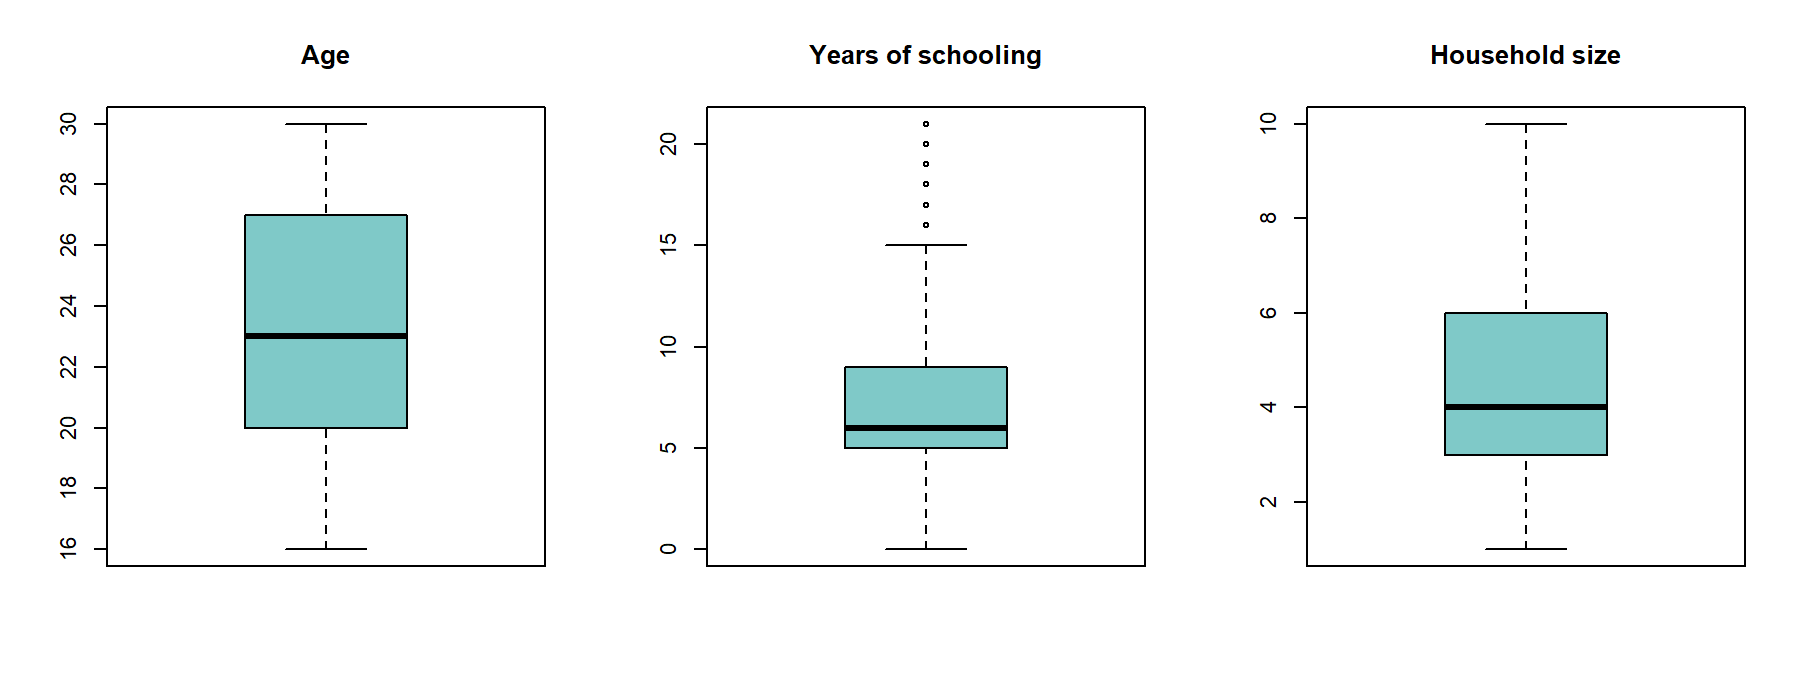
\includegraphics[width=0.85\textwidth]{eda_outliers_boxplots.png}
\caption{Box plots of the numeric variables used to detect outliers.}
\label{fig:box}
\end{figure}

\paragraph{Other preparation.} Category labels were cleaned (spelling and numbering), rare categories
were merged so that every group contains enough people, and the target was coded with
``Unemployed'' as the positive class.

\subsection{Feature engineering and selection}
Feature selection followed three rules.
\begin{enumerate}
\item \textbf{No data leakage.} Variables that are only known because a person is employed or
      unemployed (occupation, industry, hours worked, income, unemployment duration, job-search
      method, NEET status, etc.) were excluded because they directly reveal the answer.
\item \textbf{No redundancy.} Association between categorical predictors was measured with
      Cram\'er's $V$,
      \begin{equation}
      V=\sqrt{\frac{\chi^2}{n\,(\min(r,c)-1)}},
      \end{equation}
      where $\chi^2$ is the Pearson chi-square statistic of the $r\times c$ contingency table and $n$
      the sample size; numeric variables were grouped into four classes (Figure~\ref{fig:cramer}).
      Province and district are perfectly associated ($V=1.00$) because each district belongs to one
      province, so province was dropped and the more detailed district retained. Education level
      and years of schooling are also strongly related ($V=0.98$) but both were kept: they carry
      slightly different information (level completed versus time in school), and penalized and
      tree-based models handle correlated inputs well.
\item \textbf{Identifiers removed.} Household identifiers and survey-design variables are not
      predictors.
\end{enumerate}

\begin{figure}[H]
\centering
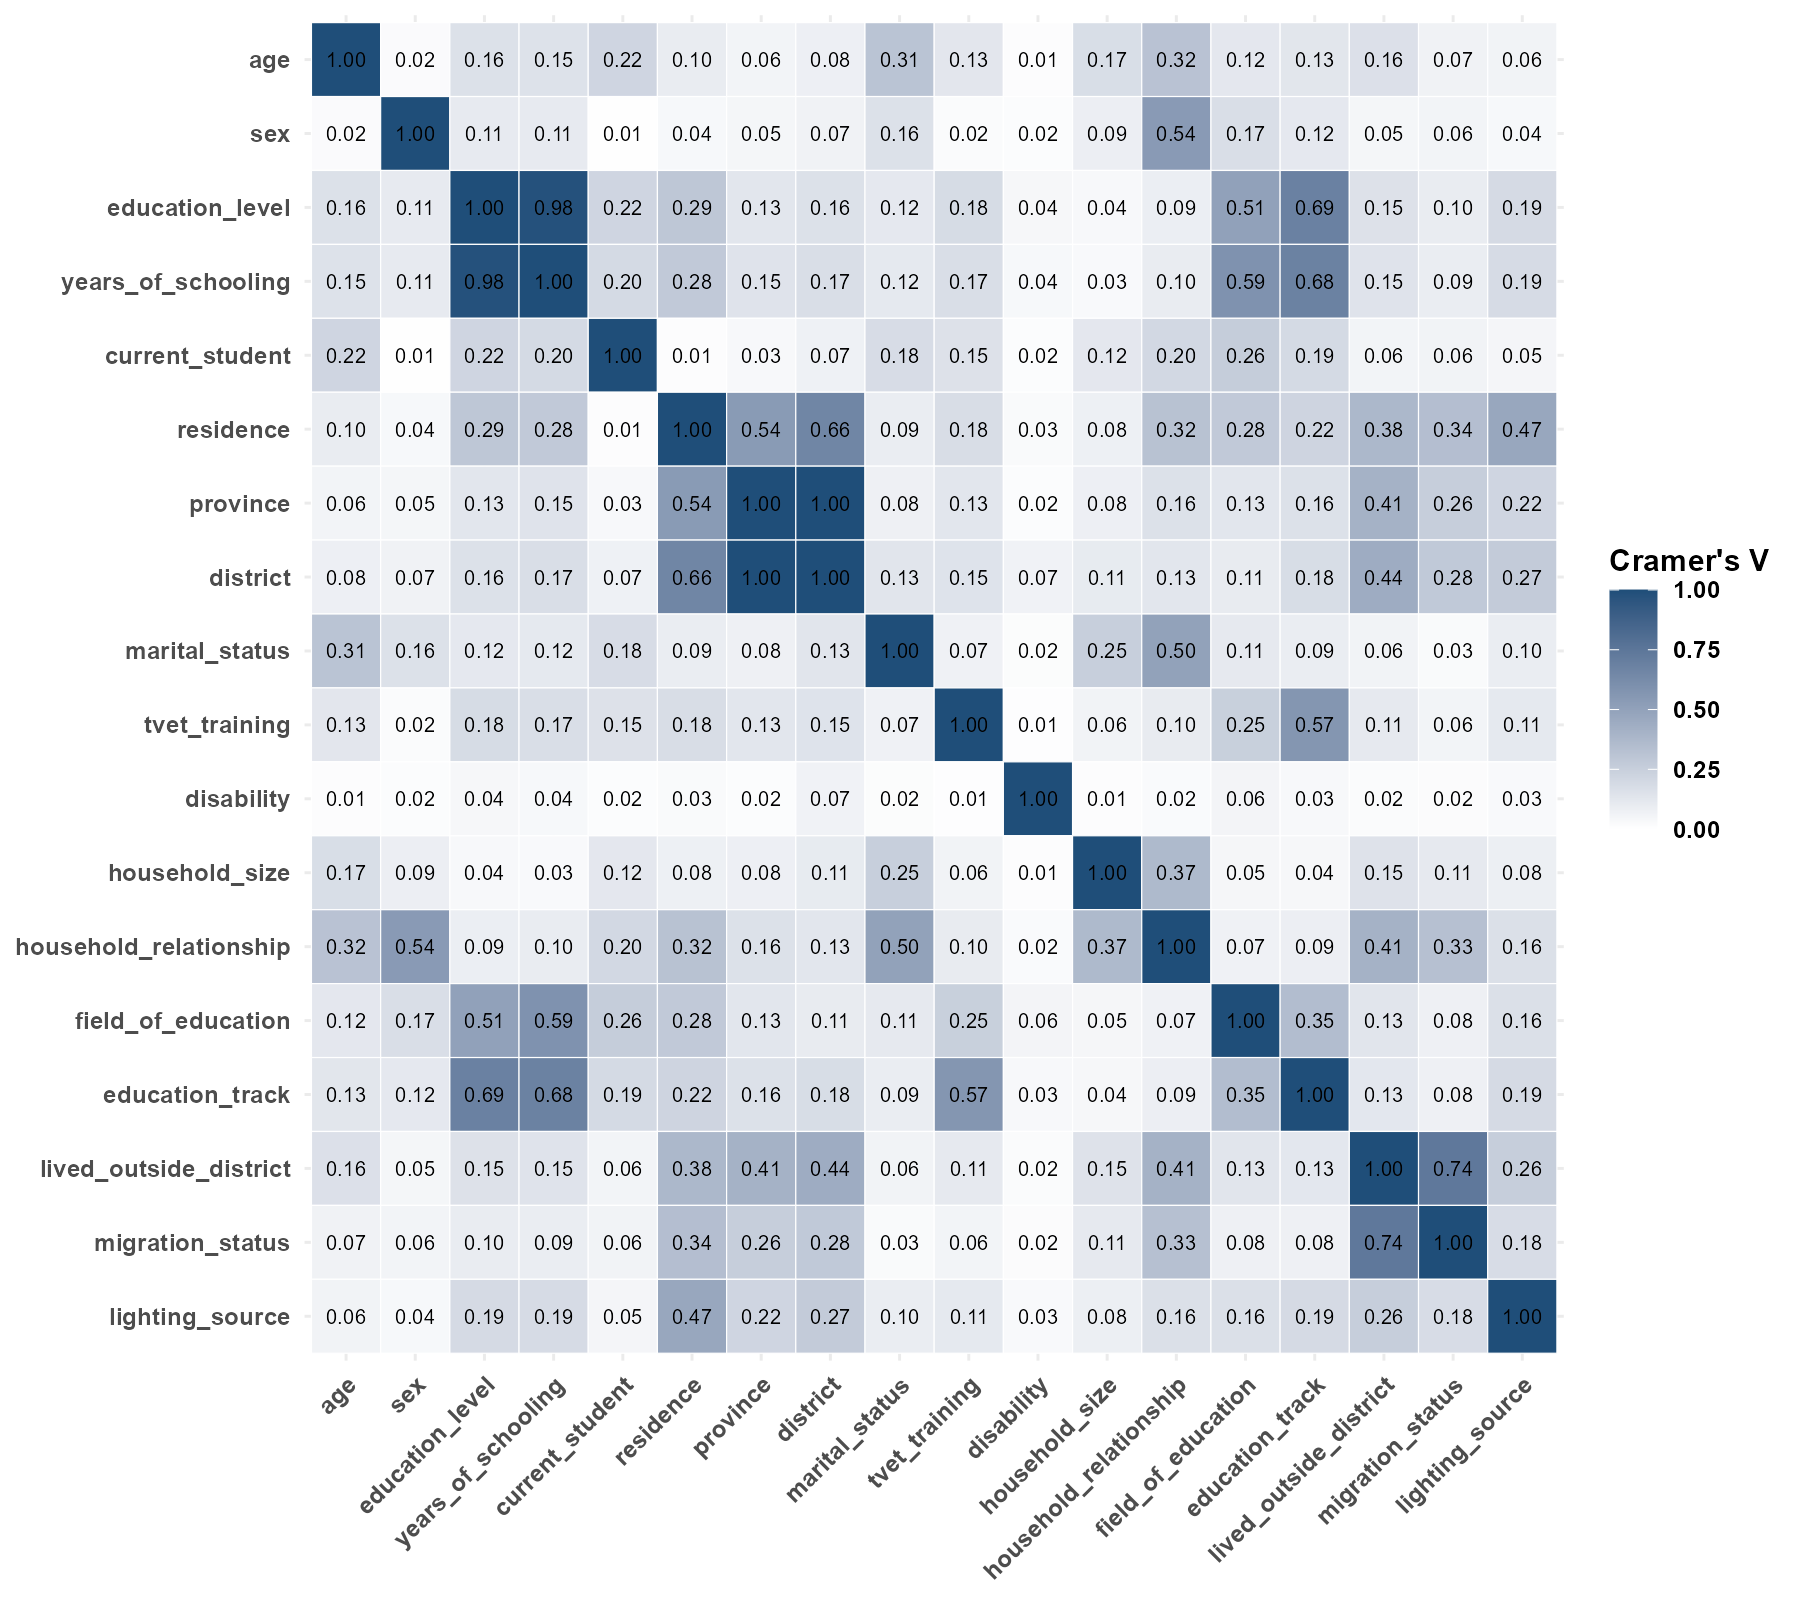
\includegraphics[width=0.82\textwidth]{report_cramers_v.png}
\caption{Association between predictors measured with Cram\'er's $V$ (0 = none, 1 = perfect).}
\label{fig:cramer}
\end{figure}

Figure~\ref{fig:edusex} shows a key pattern from the exploratory analysis: unemployment rises with
education up to upper secondary level and is higher for women at every education level.

\begin{figure}[H]
\centering
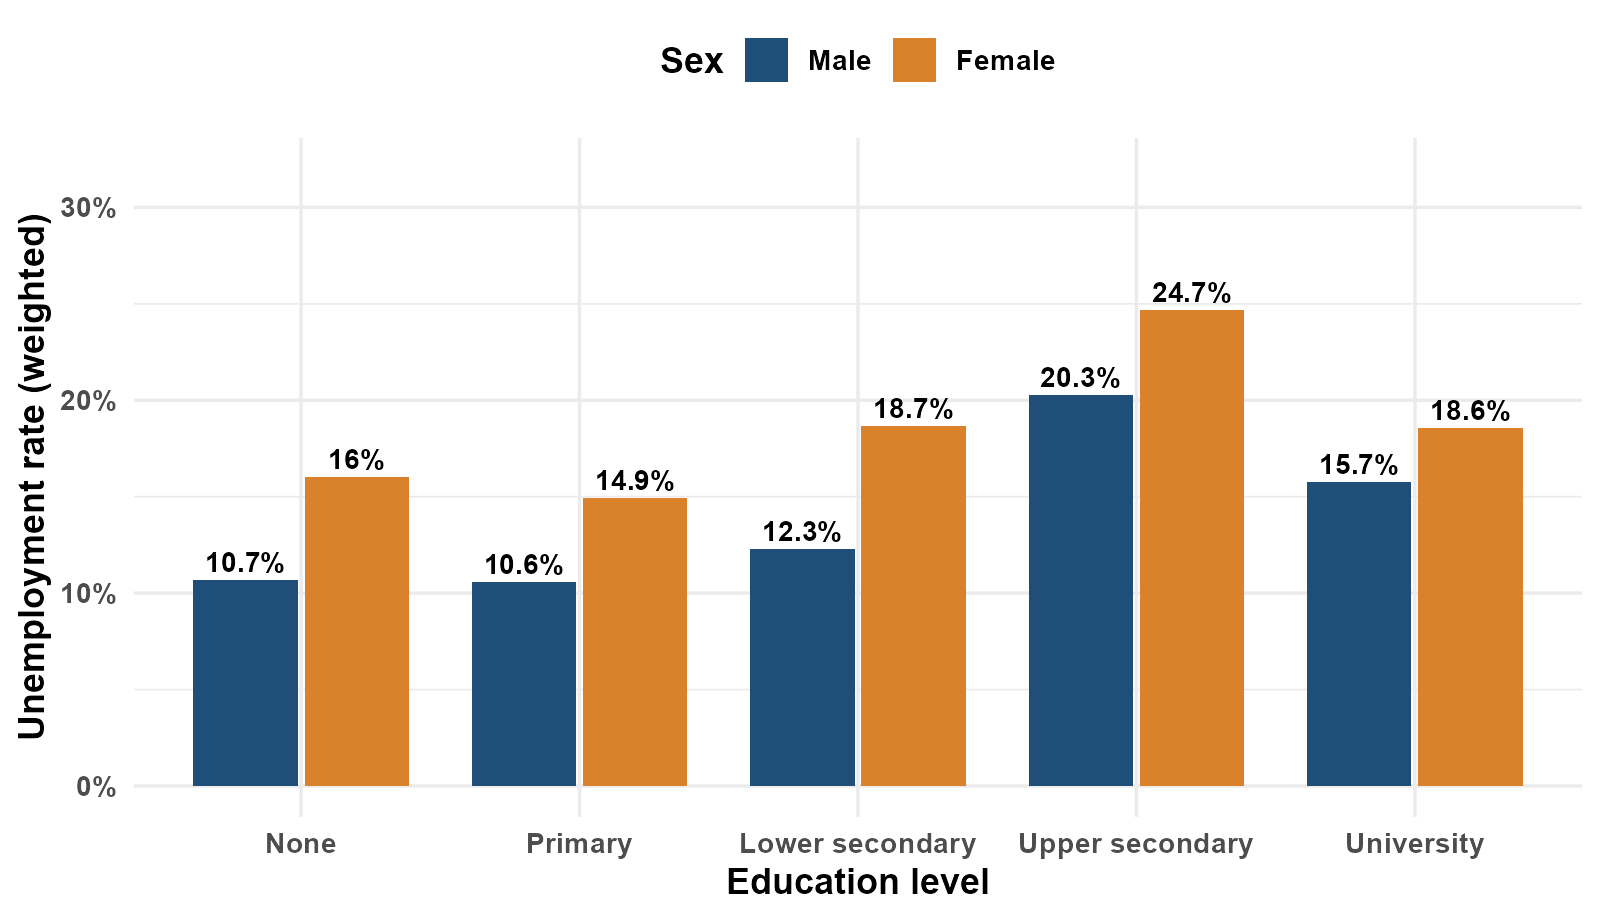
\includegraphics[width=0.82\textwidth]{report_rate_education_sex.png}
\caption{Youth unemployment rate by education level and sex (survey-weighted).}
\label{fig:edusex}
\end{figure}

\subsection{Train/test split}
The data were split by \textbf{stratified random sampling} into a \textbf{70\% training set (11{,}172
youth)} and a \textbf{30\% test set (4{,}786 youth)}. Stratification keeps the same share of
unemployed youth (14.7\%) in both sets, and a fixed random seed (123) makes the split reproducible.
The test set was used only once, at the end, to evaluate the final models. Within the training set,
\textbf{5-fold cross-validation} was used for tuning, and all ten models used exactly the same folds
so that their results are directly comparable.

To deal with class imbalance, each training fold was \textbf{down-sampled}: the employed group was
randomly reduced to the size of the unemployed group, so the models learn from balanced data.
Down-sampling is applied only inside training folds; the test set keeps the real 14.7\% rate. Because
a model trained on balanced data over-states probabilities, the web application converts a score $s$
back to a real-world chance using the true unemployment share $\pi=0.147$:
\begin{equation}
P(\text{unemployed}) = \frac{s\,\pi}{s\,\pi+(1-s)(1-\pi)}.
\label{eq:prior}
\end{equation}

% ================================================================= 4
\section{Implementation of the ML Methodology}

\subsection{Algorithms}
Table~\ref{tab:algos} lists the ten algorithms and the reason each was included. As an example of the
models' structure, the logistic regression models the log-odds of unemployment linearly,
\begin{equation}
\log\frac{P(Y=1\mid\mathbf{x})}{1-P(Y=1\mid\mathbf{x})}=\beta_0+\boldsymbol{\beta}^{\top}\mathbf{x},
\end{equation}
Lasso and elastic net add the penalty
$\lambda\big[\alpha\lVert\boldsymbol\beta\rVert_1+\tfrac{1-\alpha}{2}\lVert\boldsymbol\beta\rVert_2^2\big]$
($\alpha=1$ for Lasso), and the random forest averages the votes of many decision trees, each grown on
a bootstrap sample with a random subset of $m_{\text{try}}$ predictors considered at every split
\cite{breiman}.

\begin{table}[H]
\centering
\caption{The ten algorithms implemented and their justification}
\label{tab:algos}
\small
\rowcolors{2}{lightrow}{white}
\begin{tabularx}{\textwidth}{@{}l l Y@{}}
\toprule
\textbf{Algorithm} & \textbf{Type} & \textbf{Why it was chosen} \\
\midrule
Logistic regression & Linear, probabilistic & Standard baseline for binary outcomes; gives odds ratios \\
Lasso / Elastic net & Penalized logistic & Shrinks weak predictors; handles many dummy variables and correlated inputs \\
LDA & Linear discriminant & Simple and stable linear classifier \\
RDA & Regularized discriminant & Compromise between LDA and QDA; robust with many categories \\
Naive Bayes & Probabilistic & Very fast; useful simple benchmark \\
$k$-nearest neighbours & Instance-based & Non-parametric; no assumption on the shape of the boundary \\
Decision tree (CART) & Tree & Easy to interpret; captures interactions \\
Random forest \cite{breiman} & Ensemble of trees & Robust; handles non-linear effects and interactions \\
Gradient boosting (GBM) \cite{friedman} & Boosted trees & Often the most accurate method on tabular data \\
\bottomrule
\end{tabularx}
\end{table}

\subsection{Training and hyper-parameter tuning}
Each model was tuned by grid search with 5-fold cross-validation; the combination with the highest
mean cross-validated ROC AUC was selected (Table~\ref{tab:tune}). Figure~\ref{fig:tune} shows the
tuning surface of the random forest: the best setting considers $m_{\text{try}}=4$ predictors at each
split with a minimum node size of 30. Differences between settings are small (0.666--0.673), so the
random forest is stable with respect to its hyper-parameters.

\begin{table}[H]
\centering
\caption{Hyper-parameter tuning results (5-fold cross-validation)}
\label{tab:tune}
\small
\rowcolors{2}{lightrow}{white}
\begin{tabularx}{\textwidth}{@{}l Y c l c@{}}
\toprule
\textbf{Model} & \textbf{Parameters tuned} & \textbf{Grid size} & \textbf{Best values} & \textbf{CV ROC AUC} \\
\midrule
Random forest & $m_{\text{try}}$, minimum node size & 12 & $m_{\text{try}}=4$, node size $=30$ & 0.673 \\
GBM & number of trees, tree depth & 9 & 100 trees, depth 3 & 0.673 \\
RDA & $\gamma$, $\lambda$ & 9 & $\gamma=0.1$, $\lambda=0.5$ & 0.668 \\
Lasso & $\lambda$ ($\alpha=1$) & 10 & $\lambda=0.01$ & 0.668 \\
Elastic net & $\alpha$, $\lambda$ & 50 & $\alpha=0$, $\lambda=0.1$ & 0.667 \\
LDA & none & 1 & -- & 0.661 \\
Logistic regression & none & 1 & -- & 0.658 \\
Naive Bayes & Laplace smoothing (fixed) & 1 & Laplace $=1$ & 0.649 \\
Decision tree & complexity $c_p$ & 10 & $c_p=0.00085$ & 0.637 \\
KNN & number of neighbours $k$ & 8 & $k=41$ & 0.625 \\
\bottomrule
\end{tabularx}
\end{table}

\begin{figure}[H]
\centering
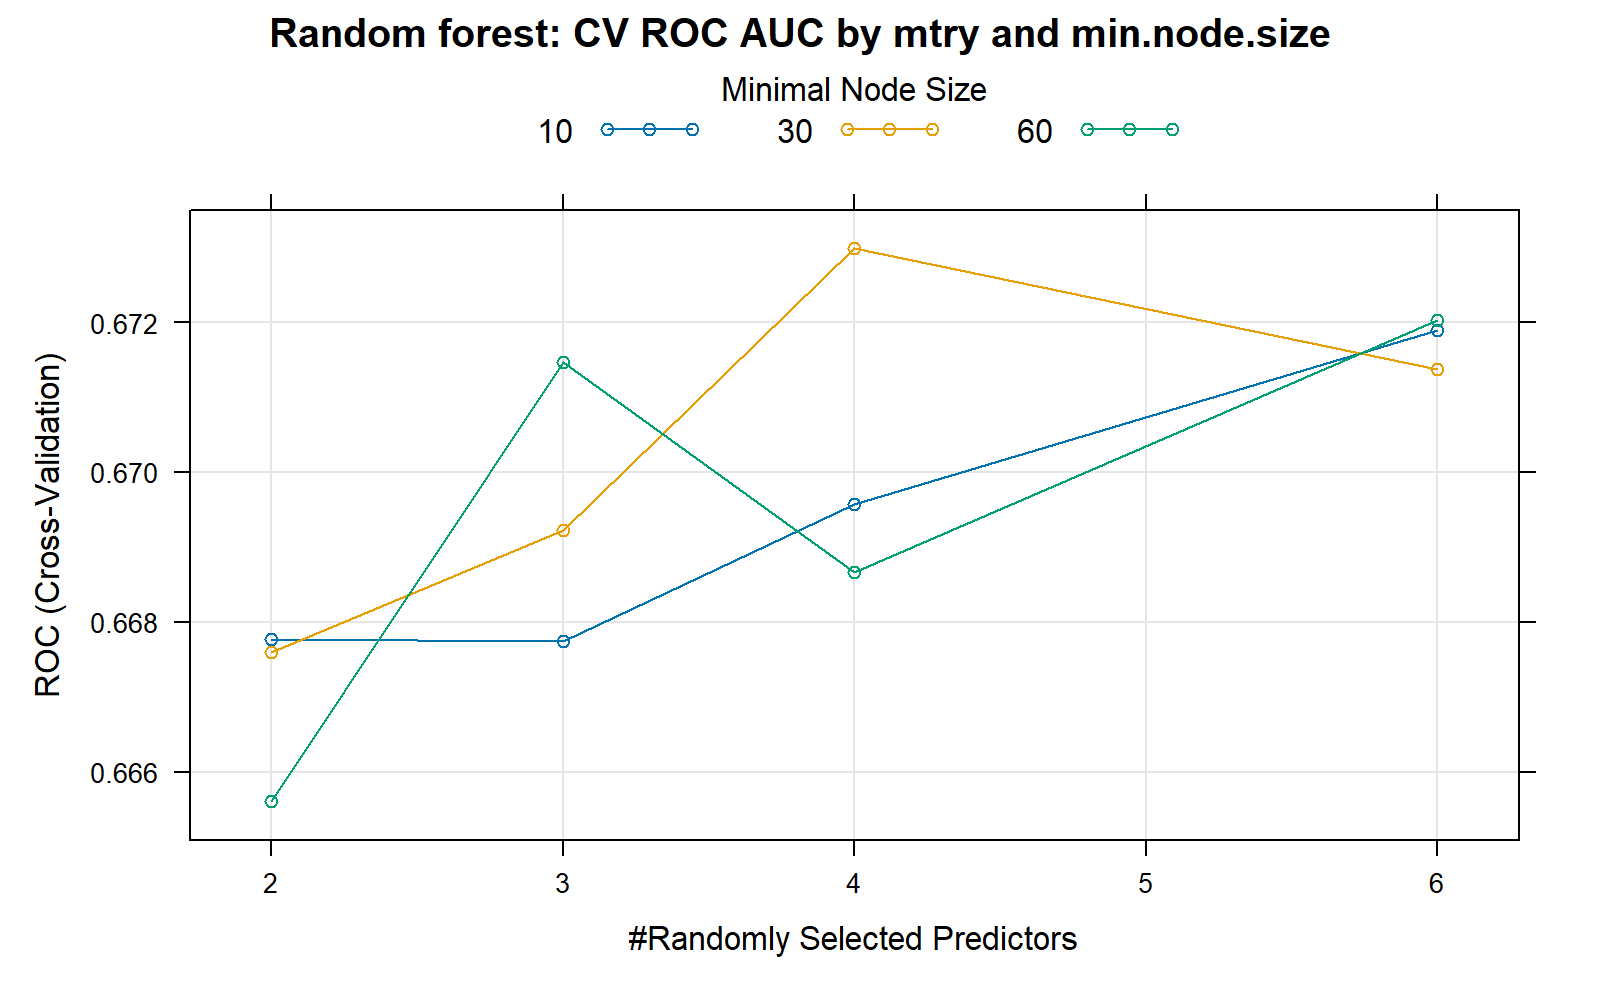
\includegraphics[width=0.78\textwidth]{04_tuning_random_forest.png}
\caption{Random forest tuning: cross-validated ROC AUC by $m_{\text{try}}$ and minimum node size.}
\label{fig:tune}
\end{figure}

\subsection{Results}
Table~\ref{tab:test} and Figure~\ref{fig:roc} present the performance of all models on the test set.
The \textbf{random forest has the highest ROC AUC (0.676)}, followed closely by GBM (0.672) and LDA
(0.664). All models clearly beat random guessing, but none is very strong. The models differ mainly in
how they balance recall and specificity: Lasso finds the most unemployed youth (recall 0.78) at the
cost of more false alarms, while RDA and the random forest are more balanced. Precision is low for
every model (about 0.2) because only 15\% of youth are unemployed.

\begin{table}[H]
\centering
\caption{Performance of all models on the test set (4{,}786 youth; cut-off 0.5)}
\label{tab:test}
\small
\begin{tabularx}{\textwidth}{@{}Y c c c c c c c@{}}
\toprule
\textbf{Model} & \textbf{ROC AUC} & \textbf{Accuracy} & \textbf{Recall} & \textbf{Specificity} & \textbf{Precision} & \textbf{$F_1$} & \textbf{$\kappa$} \\
\midrule
\rowcolor{bestrow}\textbf{Random forest} & \textbf{0.676} & 0.623 & 0.621 & 0.624 & 0.222 & 0.327 & 0.140 \\
GBM & 0.672 & 0.565 & 0.708 & 0.540 & 0.210 & 0.324 & 0.125 \\
\rowcolor{lightrow}LDA & 0.664 & 0.577 & 0.685 & 0.558 & 0.211 & 0.323 & 0.126 \\
RDA & 0.662 & 0.644 & 0.560 & 0.658 & 0.221 & 0.317 & 0.133 \\
\rowcolor{lightrow}Lasso & 0.660 & 0.518 & 0.782 & 0.472 & 0.204 & 0.323 & 0.117 \\
Logistic regression & 0.656 & 0.570 & 0.684 & 0.550 & 0.208 & 0.319 & 0.120 \\
\rowcolor{lightrow}Elastic net & 0.656 & 0.575 & 0.685 & 0.556 & 0.211 & 0.322 & 0.125 \\
Naive Bayes & 0.647 & 0.621 & 0.567 & 0.630 & 0.209 & 0.306 & 0.115 \\
\rowcolor{lightrow}Decision tree & 0.640 & 0.576 & 0.627 & 0.567 & 0.200 & 0.303 & 0.103 \\
KNN & 0.627 & 0.547 & 0.647 & 0.529 & 0.192 & 0.296 & 0.089 \\
\midrule
Always ``Employed'' & 0.500 & 0.853 & 0.000 & 1.000 & -- & -- & 0.000 \\
\bottomrule
\end{tabularx}
\end{table}

\begin{figure}[H]
\centering
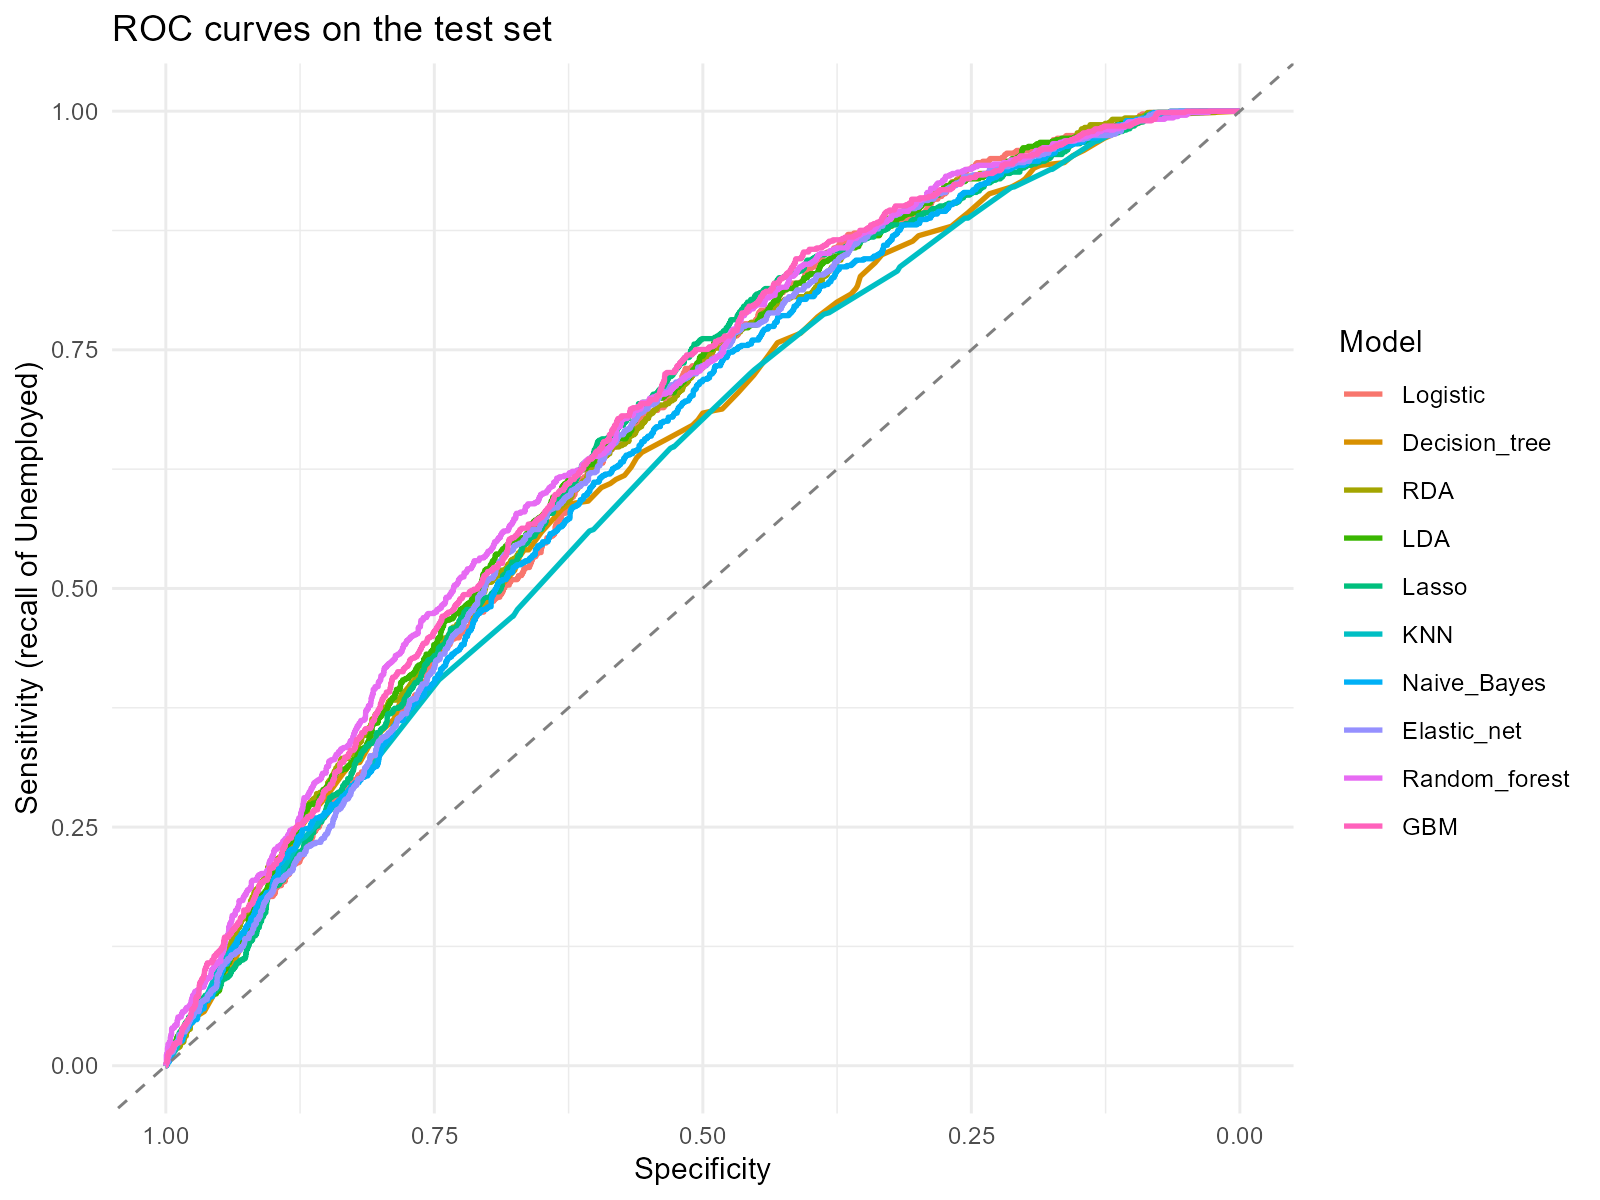
\includegraphics[width=0.74\textwidth]{02_roc_curves.png}
\caption{ROC curves of the ten models on the test set; the dashed diagonal is random guessing.}
\label{fig:roc}
\end{figure}

\paragraph{Confusion matrix of the best model.} Table~\ref{tab:cm} shows that, of the 705 unemployed
youth in the test set, the random forest correctly identified 438 (62\%) and missed 267, while it
wrongly flagged 1{,}536 employed youth. When the model predicts that a young person is employed it is
right 90.5\% of the time (negative predictive value), so it is most useful for screening: setting
aside low-risk youth and short-listing high-risk youth for further attention.

\begin{table}[H]
\centering
\caption{Confusion matrix of the random forest on the test set (cut-off 0.5)}
\label{tab:cm}
\begin{tabularx}{0.85\textwidth}{@{}l Y Y r@{}}
\toprule
 & \textbf{Predicted unemployed} & \textbf{Predicted employed} & \textbf{Total} \\
\midrule
\textbf{Actually unemployed} & 438 (found) & 267 (missed) & 705 \\
\rowcolor{lightrow}\textbf{Actually employed} & 1{,}536 (false alarm) & 2{,}545 (correct) & 4{,}081 \\
\midrule
\textbf{Total} & 1{,}974 & 2{,}812 & 4{,}786 \\
\bottomrule
\end{tabularx}
\end{table}

\paragraph{Feature importance.} Figure~\ref{fig:imp} ranks the variables used by the random forest.
District, relationship to the household head, age, years of schooling and household size dominate,
followed by lighting source (a proxy for household living standard), education level and field of
education. This impurity-based importance tends to favour variables with many distinct values, such
as district (30 levels) and age, so it should be read together with the direction of effects below.

\begin{figure}[H]
\centering
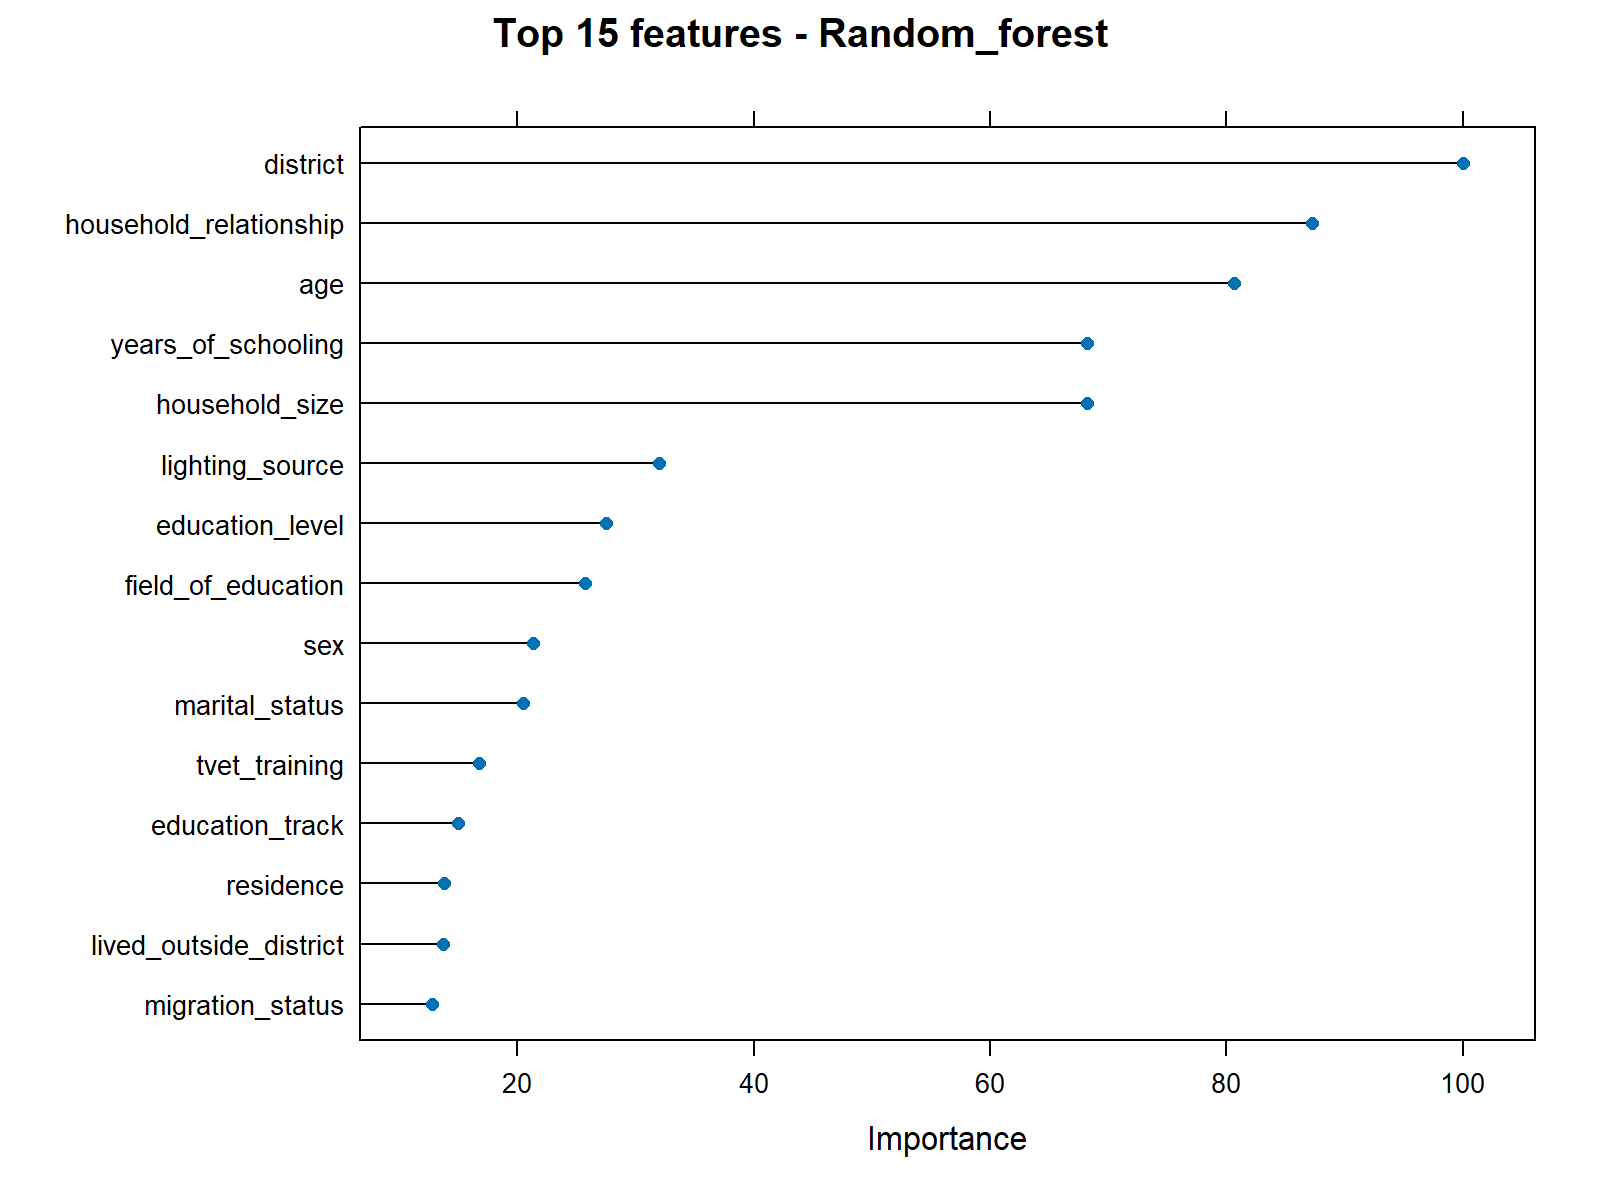
\includegraphics[width=0.74\textwidth]{03_feature_importance.png}
\caption{Top 15 predictors in the random forest (importance scaled from 0 to 100).}
\label{fig:imp}
\end{figure}

\paragraph{Direction of effects.} Importance shows \emph{which} variables matter, not \emph{how}. Two
tools were therefore used. First, the logistic regression gives odds ratios of unemployment,
$\mathrm{OR}_j=e^{\beta_j}$ (Table~\ref{tab:or}); an odds ratio below one means lower odds than the
reference group, holding the other variables constant. Second, partial dependence plots of the random
forest show how the average risk score changes with one variable while the other variables keep their
observed values (Figures~\ref{fig:pdp1} and~\ref{fig:pdp2}).

\begin{table}[H]
\centering
\caption{Odds ratios of being unemployed (logistic regression; $p<0.05$; districts not shown)}
\label{tab:or}
\small
\rowcolors{2}{lightrow}{white}
\begin{tabularx}{\textwidth}{@{}Y c c c l@{}}
\toprule
\textbf{Characteristic (reference group)} & \textbf{OR} & \textbf{95\% CI} & \textbf{$p$-value} & \textbf{Interpretation} \\
\midrule
Household head (vs brother/sister of head) & 0.31 & 0.17--0.54 & $<0.001$ & about 70\% lower odds \\
Non-relative (vs brother/sister of head) & 0.48 & 0.25--0.93 & 0.028 & about 52\% lower odds \\
Single (vs living together) & 0.56 & 0.38--0.83 & 0.004 & about 44\% lower odds \\
Male (vs female) & 0.77 & 0.64--0.93 & 0.006 & 23\% lower odds than women \\
\bottomrule
\end{tabularx}
\end{table}

Children of the household head (OR 1.13) and married youth (OR 0.93) do not differ significantly from
their reference groups. Seven districts (Nyabihu, Gakenke, Kayonza, Ngoma, Kirehe, Nyagatare and
Nyarugenge) have significantly lower odds than the reference district, Bugesera. After adjustment,
education level is not individually significant in the linear logistic model, but the flexible random
forest captures a clear threshold effect of schooling (Figure~\ref{fig:pdp1}a).

\begin{figure}[H]
\centering
\begin{subfigure}{0.49\textwidth}\centering
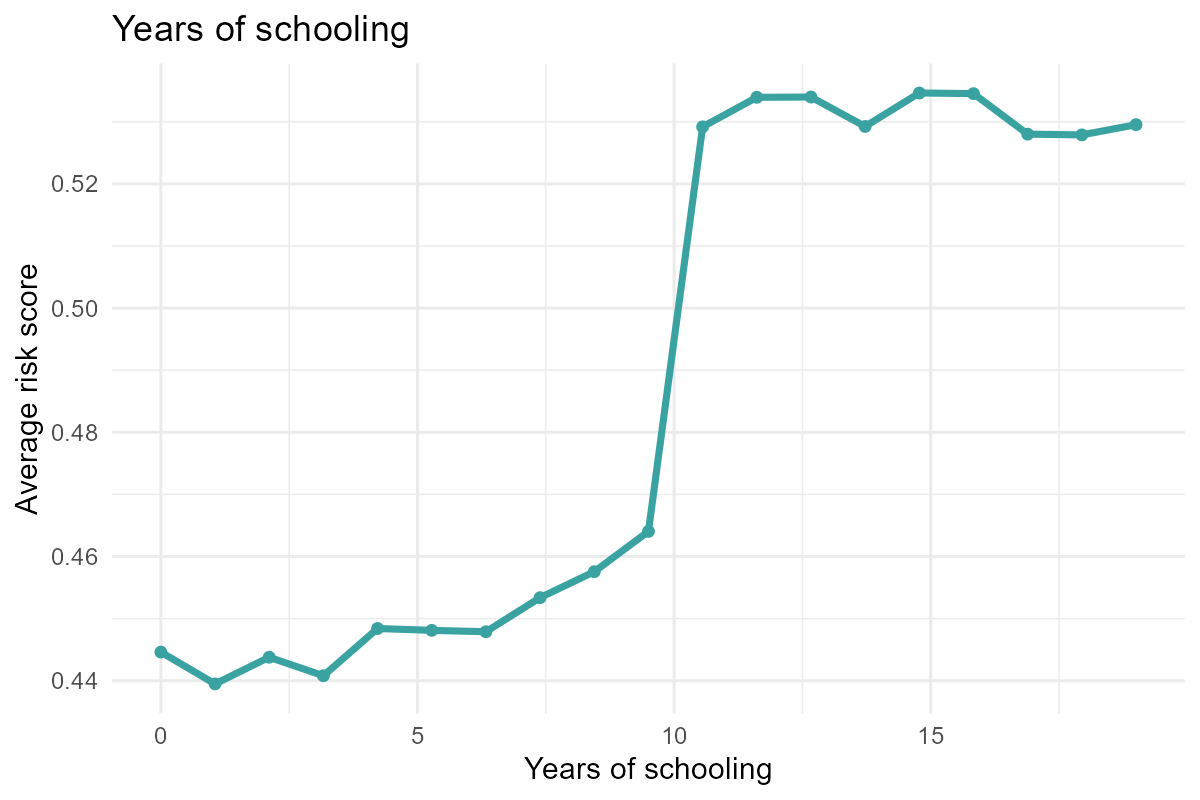
\includegraphics[width=\linewidth]{10_pdp_schooling.png}\caption{Years of schooling}\end{subfigure}
\hfill
\begin{subfigure}{0.49\textwidth}\centering
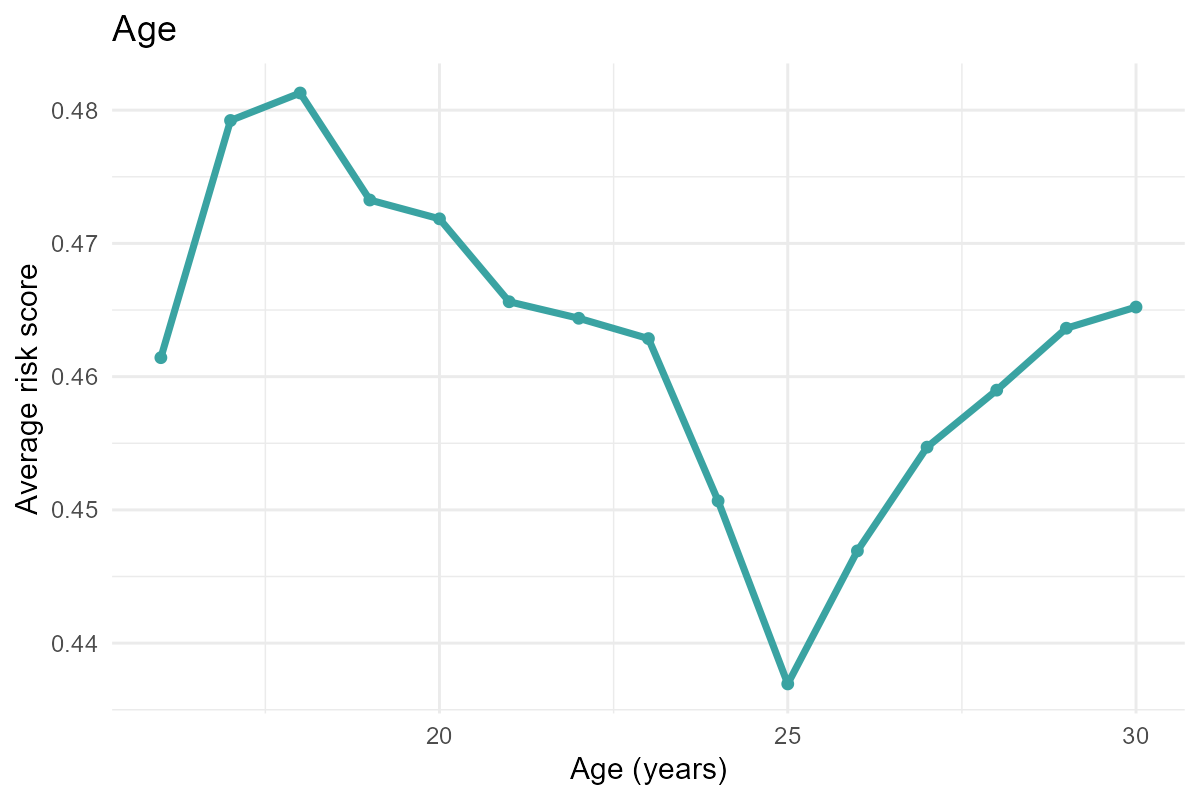
\includegraphics[width=\linewidth]{11_pdp_age.png}\caption{Age}\end{subfigure}
\caption{Partial dependence of the random-forest risk score on schooling and age.}
\label{fig:pdp1}
\end{figure}

\begin{figure}[H]
\centering
\begin{subfigure}{0.49\textwidth}\centering
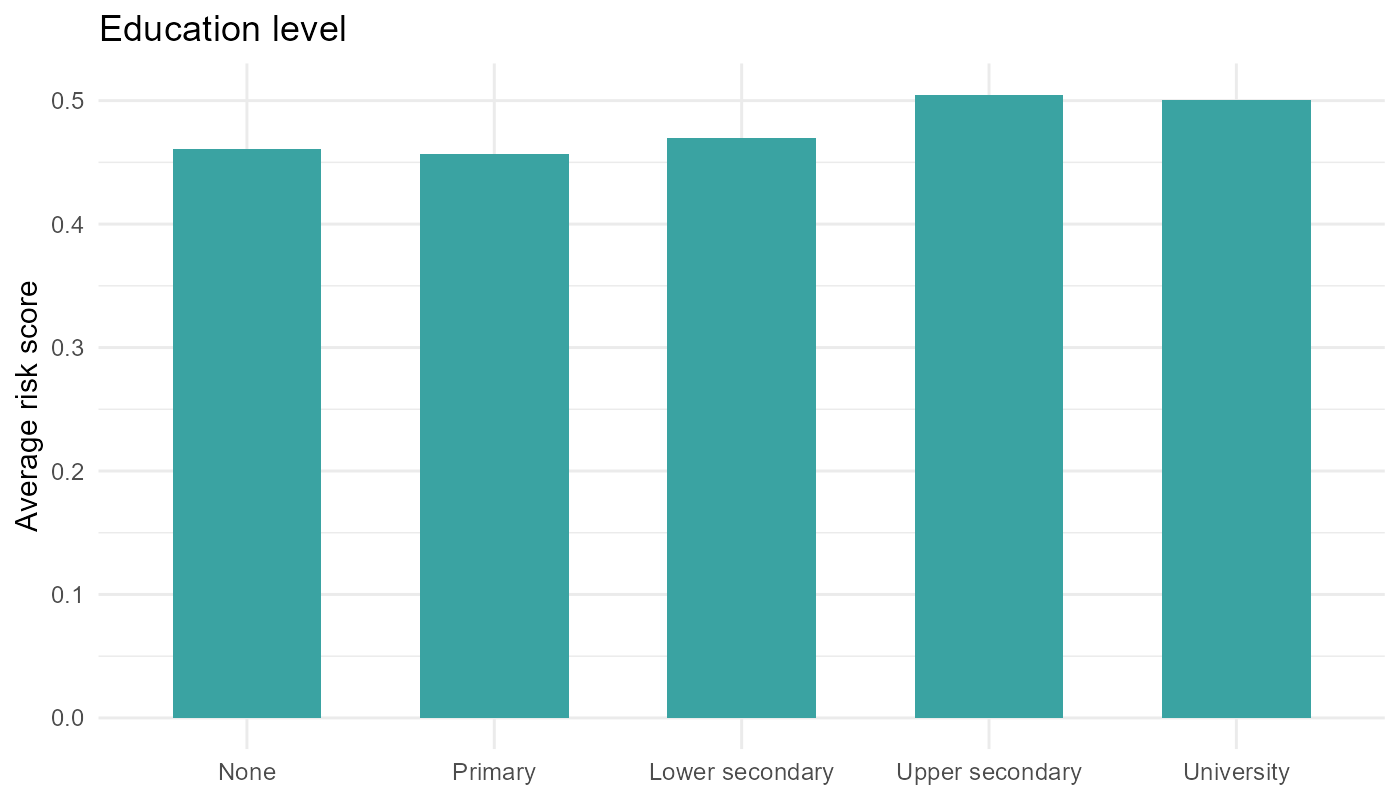
\includegraphics[width=\linewidth]{14_pdp_education.png}\caption{Education level}\end{subfigure}
\hfill
\begin{subfigure}{0.49\textwidth}\centering
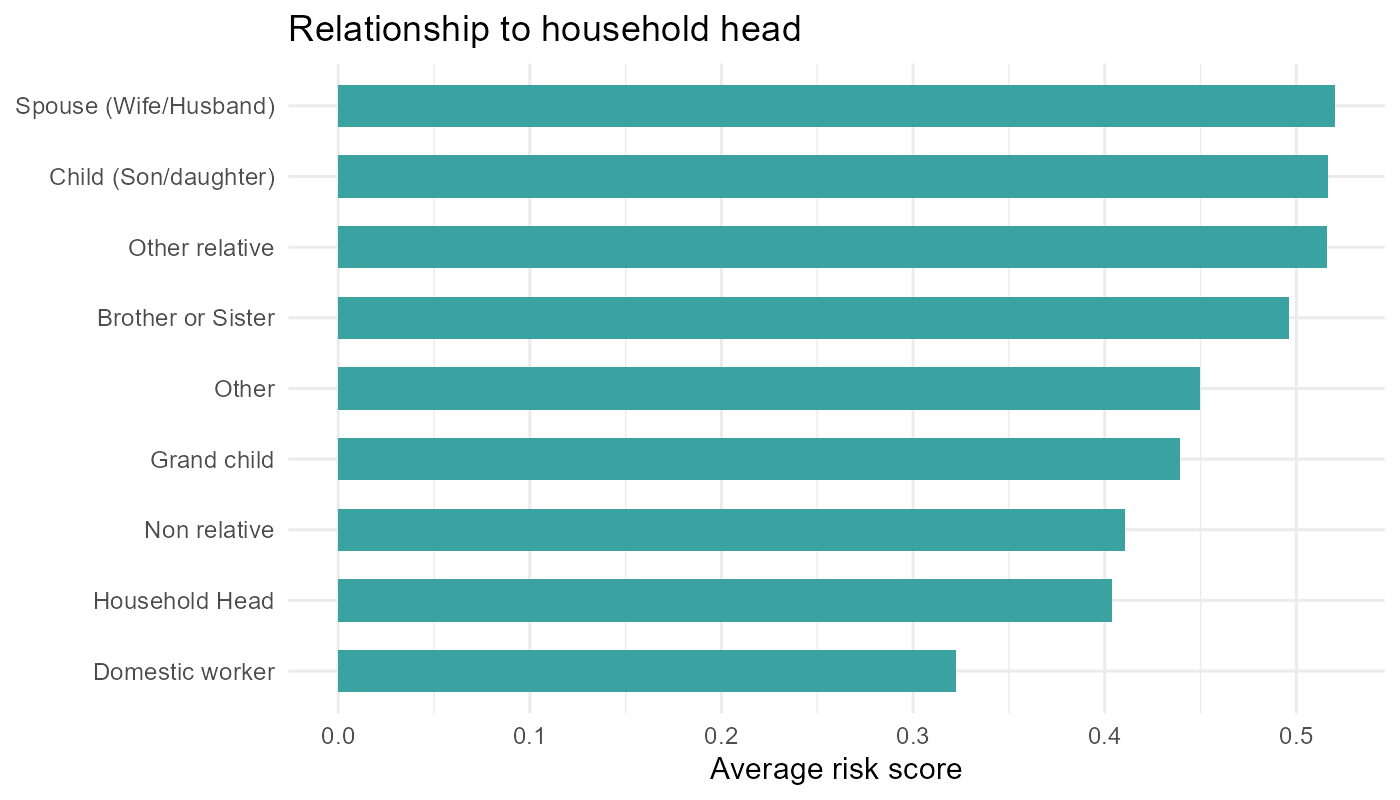
\includegraphics[width=\linewidth]{15_pdp_relationship.png}\caption{Relationship to household head}\end{subfigure}
\caption{Partial dependence of the random-forest risk score on education level and household position.}
\label{fig:pdp2}
\end{figure}

The risk of unemployment is almost flat up to about nine years of schooling and then \textbf{jumps
sharply after ten years} (the end of lower secondary), remaining high for upper secondary and
university levels. By age, risk peaks at 17--18 years, falls to its lowest level around 25, and then
rises slightly. Household heads and domestic workers have the lowest risk. These patterns agree with
the descriptive rates in Table~\ref{tab:rates} and Figure~\ref{fig:edusex}.

\subsection{Testing, verification and validation}
The final models were validated in three complementary ways.

\paragraph{(a) Cross-validation versus test set.} Figure~\ref{fig:cv} shows the mean cross-validated
ROC AUC of each model with its 95\% confidence interval. The random forest and GBM have the best CV
score (0.673), and the random forest's test ROC AUC (0.676) is almost identical. This close agreement
shows that the models are \textbf{not overfitting} and that the result is not due to a lucky split.

\begin{figure}[H]
\centering
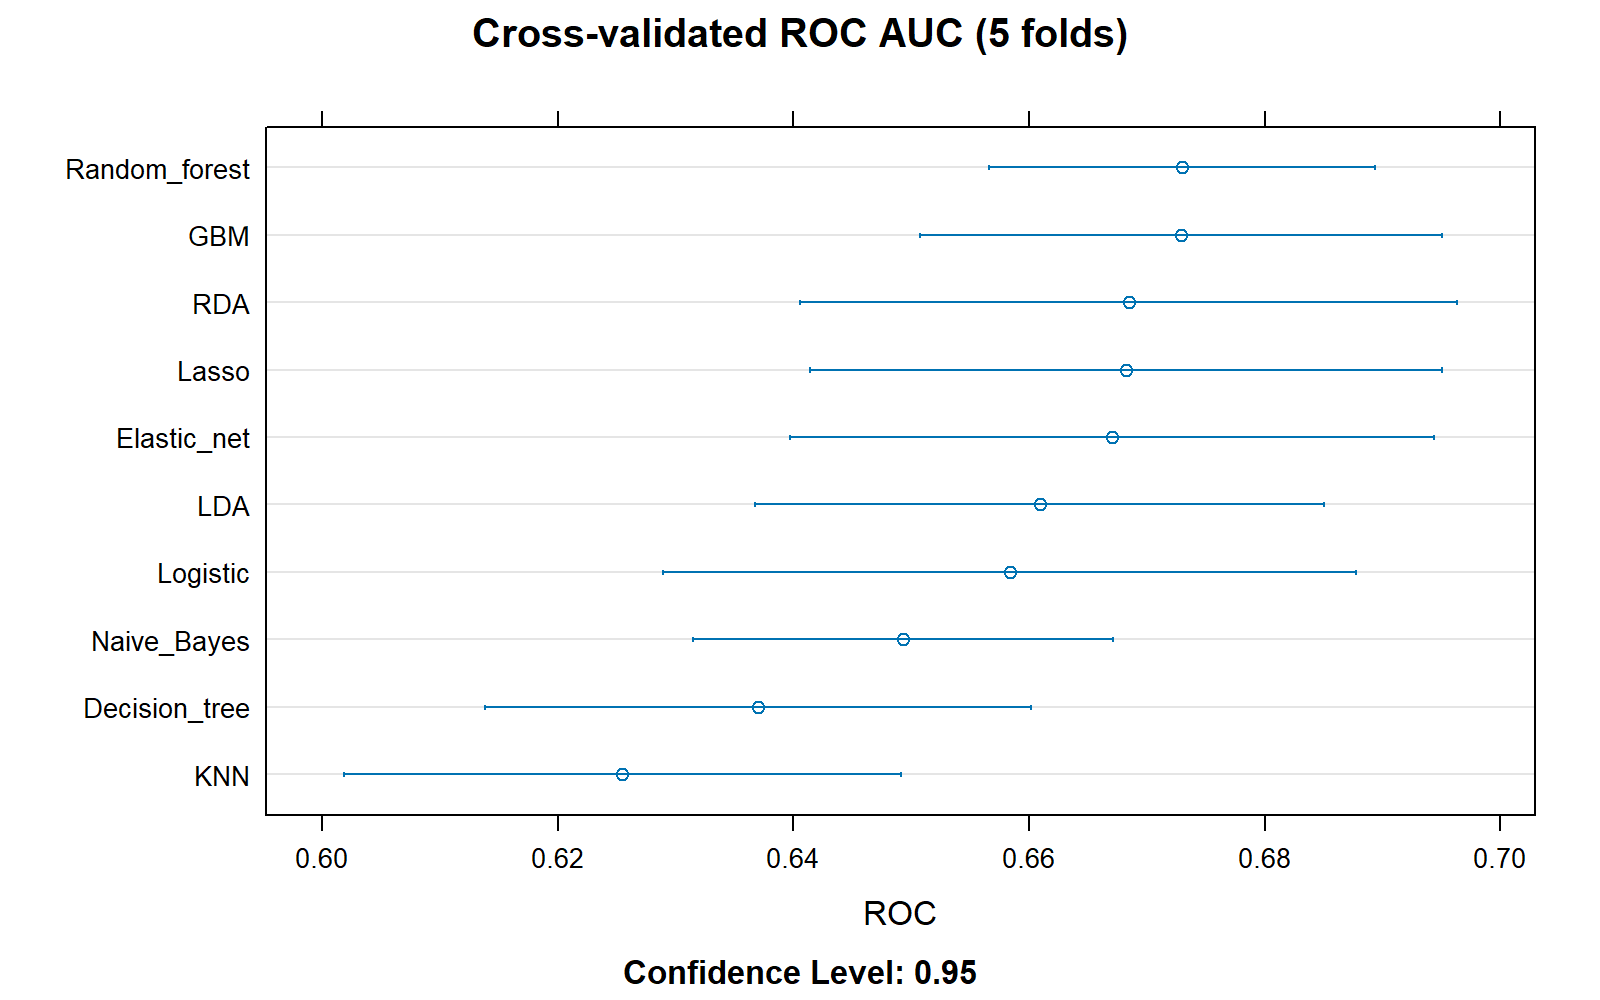
\includegraphics[width=0.8\textwidth]{01_cv_comparison.png}
\caption{Cross-validated ROC AUC of the ten models (5 folds; dot = mean, bar = 95\% confidence interval).}
\label{fig:cv}
\end{figure}

\paragraph{(b) Statistical significance.} Table~\ref{tab:delong} compares the random forest with
other models using the DeLong test on the same test set. The random forest is significantly better
than logistic regression and KNN, but \textbf{not significantly better than GBM, LDA or Lasso}. The
95\% confidence interval of its ROC AUC is 0.656--0.696. In practice the four best models perform
about equally well; the random forest was chosen for the web application because it has the highest
score.

\begin{table}[H]
\centering
\caption{DeLong tests comparing ROC curves on the test set}
\label{tab:delong}
\rowcolors{2}{lightrow}{white}
\begin{tabularx}{\textwidth}{@{}Y c c l@{}}
\toprule
\textbf{Comparison} & \textbf{AUC difference} & \textbf{$p$-value} & \textbf{Significant at 5\%?} \\
\midrule
Random forest vs GBM & 0.004 & 0.587 & No \\
Random forest vs LDA & 0.011 & 0.198 & No \\
Random forest vs Lasso & 0.016 & 0.056 & No (borderline) \\
Random forest vs Logistic regression & 0.019 & 0.038 & Yes \\
Random forest vs KNN & 0.049 & $<0.001$ & Yes \\
\bottomrule
\end{tabularx}
\end{table}

\paragraph{(c) Performance in subgroups.} Table~\ref{tab:sub} checks whether the model works equally
well for different groups. It separates employed and unemployed youth better in urban areas (ROC AUC
0.74) than in rural areas (0.64). For women it finds most unemployed youth (recall 0.73) but raises
more false alarms (specificity 0.46), whereas for men it finds fewer than half (recall 0.48). The
model therefore behaves differently by sex, which must be taken into account before any practical use.

\begin{table}[H]
\centering
\caption{Performance of the random forest by subgroup (test set)}
\label{tab:sub}
\rowcolors{2}{lightrow}{white}
\begin{tabularx}{\textwidth}{@{}Y c c c c c@{}}
\toprule
\textbf{Group} & \textbf{Youth in test set} & \textbf{Unemployment rate} & \textbf{ROC AUC} & \textbf{Recall} & \textbf{Specificity} \\
\midrule
Female & 2{,}265 & 17.6\% & 0.638 & 0.732 & 0.458 \\
Male & 2{,}521 & 12.1\% & 0.683 & 0.477 & 0.763 \\
Urban & 1{,}794 & 13.5\% & 0.737 & 0.645 & 0.675 \\
Rural & 2{,}992 & 15.5\% & 0.636 & 0.609 & 0.592 \\
\bottomrule
\end{tabularx}
\end{table}

% ================================================================= 5
\section{Communicating Findings}

\subsection{Key findings and interpretation}
\begin{enumerate}
\item \textbf{Youth unemployment is concentrated in specific groups.} The weighted rate is 14.7\%, but
      it reaches 17.4\% for young women and 22.5\% for youth with upper secondary education.
\item \textbf{The education paradox.} Both the descriptive rates and the random forest show that risk
      rises after about ten years of schooling. Educated youth often wait for jobs that match their
      qualifications, while less educated youth quickly enter agriculture or informal work. Having a
      job does not mean having a good job, given that about 90\% of employment is informal
      \cite{nisr_annual}.
\item \textbf{Position in the household matters.} Household heads have about 70\% lower odds of
      unemployment than siblings of the head and receive the lowest risk from the random forest. Sons,
      daughters, grandchildren and spouses, who can rely on family support while searching, have the
      highest unemployment rates.
\item \textbf{Gender gap.} After controlling for education, age and location, young men still have
      23\% lower odds of unemployment than young women.
\item \textbf{Location.} District is the strongest predictor in the random forest and several
      districts differ significantly, reflecting local labour-market conditions.
\item \textbf{Prediction is possible but modest.} The best ROC AUC is about 0.68. Simple linear models
      (LDA, Lasso) are nearly as good as the random forest and GBM, so the relationships are mostly
      simple and additive. Much of what determines whether a young person finds work (networks, job
      offers, motivation, local demand) is not measured in the survey.
\end{enumerate}
For policy, the model is best used as a \textbf{screening tool} that identifies groups to prioritise
for employment services, such as young women and secondary-school leavers in high-risk districts,
rather than to make decisions about individuals.

\subsection{Limitations}
\begin{itemize}
\item \textbf{Modest predictive power} (ROC AUC $\approx 0.68$) and low precision: many youth flagged
      as at risk are actually employed.
\item \textbf{Associations, not causes.} The data are cross-sectional; the results show which
      characteristics predict unemployment, not what causes it.
\item \textbf{Survey design not used in training.} Models were trained without survey weights,
      strata or clusters; descriptive rates are weighted, but model performance describes the sample.
\item \textbf{Rotating panel.} The same household can appear in several quarters, so related records
      may fall in both training and test sets, which may make test results slightly optimistic.
\item \textbf{Importance measure.} Random-forest impurity importance favours variables with many
      levels (district, age).
\item \textbf{Scope.} Only youth in the labour force were modelled; youth outside the labour force and
      the quality of employment were not studied. The analysis uses 2025 data, whereas the related
      research proposal refers to the 2024 survey.
\item \textbf{Fairness.} Recall and specificity differ markedly between women and men.
\end{itemize}

\subsection{Potential improvements}
\begin{itemize}
\item Split the data by household (grouped cross-validation) so that related records never appear in
      both training and test sets.
\item Train with survey weights and report design-based uncertainty.
\item Choose the cut-off from the relative cost of missing an unemployed youth versus a false alarm,
      possibly with group-specific cut-offs to reduce the gender gap.
\item Add more informative variables (job-search behaviour, previous work experience, household income,
      local labour demand) and pool several survey years.
\item Use permutation importance or SHAP values for fairer variable importance.
\item Extend to a three-class model (employed, unemployed, outside the labour force), as planned in the
      research proposal.
\end{itemize}

% ================================================================= 6
\section{Bonus Task: Web Application}
An interactive dashboard, \textbf{Rwanda Youth Employment (LFS 2025)}, was developed in R with
\texttt{Shiny}, \texttt{bslib} and \texttt{plotly} (Figure~\ref{fig:app}). It runs locally from the
project folder (\texttt{App/app.R}). Its main features are:
\begin{itemize}
\item \textbf{Ten pages}: executive summary, who is unemployed, education and skills, geography,
      unemployed youth, employed youth, household and time use, model and predictions, data explorer,
      and help/glossary.
\item \textbf{Filters} by sex, residence, province, education and age, with survey weights that can be
      switched on or off; all charts, KPI cards and summary tables update immediately.
\item \textbf{Model page}: comparison table of the ten models, ROC and cross-validation charts, a
      cut-off slider that updates the confusion matrix and metrics, and the feature-importance chart.
\item \textbf{Risk calculator}: the user describes a young person and the random forest returns a risk
      score, the estimated real chance of unemployment from Equation~\eqref{eq:prior}, and how the risk
      changes with age.
\item \textbf{Usability}: dark mode, numbers on charts that can be switched off, sortable bars, PNG
      download of every chart and CSV download of the filtered data.
\end{itemize}

\begin{figure}[H]
\centering
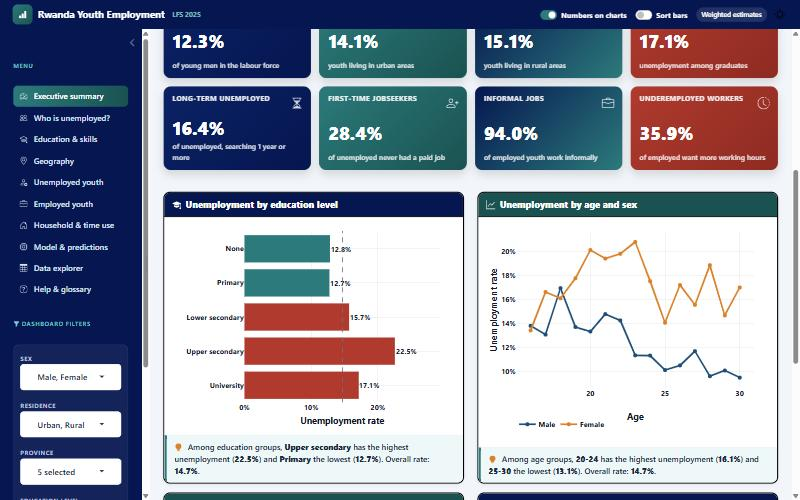
\includegraphics[width=0.95\textwidth]{dashboard_exec.jpg}
\caption{Executive summary page of the Shiny dashboard (KPI cards and first charts).}
\label{fig:app}
\end{figure}

% ================================================================= 7
\section{Conclusions}
This project translated youth unemployment in Rwanda into a binary classification task and solved it
with ten machine-learning algorithms using the 2025 Labour Force Survey. After careful cleaning,
leakage-free feature selection, a stratified 70/30 split, 5-fold cross-validation and down-sampling
for class imbalance, the \textbf{random forest} achieved the best test ROC AUC (0.676), although it was
not significantly better than GBM, LDA or Lasso. Accuracy and test error were deliberately not used to
select models, because a useless model that predicts ``employed'' for everybody would have the highest
accuracy.

The models consistently point to the same risk factors: district, position in the household, age,
schooling and sex. The clearest message is the \textbf{education paradox}: young people who complete
more than lower secondary education face a higher risk of unemployment, and young women are more
affected than young men at every level of education. These findings support policies that link
secondary and tertiary education more closely to the labour market, through career guidance,
internships and work-based learning, and that specifically target young women. The modest predictive
power also shows the limits of household-survey data for predicting individual outcomes and the need
for richer data on job search and local labour demand. The interactive web application makes these
results accessible to policy makers, students and other stakeholders.

% ================================================================= REFERENCES
\begin{thebibliography}{99}
\addcontentsline{toc}{section}{References}
\small
\bibitem{nisr_q2} National Institute of Statistics of Rwanda (NISR). (2026). \emph{Labour Force Survey 2026 (Q2): May 2026}. Kigali: NISR.
\bibitem{nisr_q3} NISR. (2026). \emph{Labour Force Survey 2026 (Q3): August 2026}. Kigali: NISR.
\bibitem{nisr_annual} NISR. (2025). \emph{Labour Force Survey Annual Report 2024}. Kigali: NISR.
\bibitem{worldbank} World Bank. (2026, February 23). \emph{Rwanda's skills training delivers jobs and opportunity for youth}. World Bank Results Brief.
\bibitem{nisr_micro25} NISR. (2026). \emph{Rwanda Labour Force Survey 2025: Microdata catalogue}, Study RWA-NISR-RLFS-2025-v0.1. https://microdatabk.statistics.gov.rw/catalog/125.
\bibitem{nisr_dict} NISR. (2025). \emph{Rwanda Labour Force Survey 2024: Microdata catalogue and data dictionary}. Kigali: NISR.
\bibitem{nisr_method} NISR. (2024). \emph{Labour Force Survey: Methodology (2024 revision)}. Kigali: NISR.
\bibitem{ilo} International Labour Organization. (2013). \emph{Resolution concerning statistics of work, employment and labour underutilization}. 19th International Conference of Labour Statisticians, Geneva.
\bibitem{ndagijimana} Ndagijimana, J., Nzasingizimana, T., \& Heshmati, A. (2018). An analysis of the determinants of youth employment in Rwanda. \emph{UKH Journal of Social Sciences}, 2(2), 1--10.
\bibitem{afdb} African Development Bank. (2014). \emph{Analysis of gender and youth employment in Rwanda}. Economic Brief.
\bibitem{becker} Becker, G. S. (1993). \emph{Human Capital: A Theoretical and Empirical Analysis, with Special Reference to Education} (3rd ed.). University of Chicago Press.
\bibitem{mincer} Mincer, J. A. (1974). \emph{Schooling, Experience, and Earnings}. National Bureau of Economic Research.
\bibitem{islr} James, G., Witten, D., Hastie, T., \& Tibshirani, R. (2021). \emph{An Introduction to Statistical Learning with Applications in R} (2nd ed.). Springer.
\bibitem{kuhn_johnson} Kuhn, M., \& Johnson, K. (2013). \emph{Applied Predictive Modeling}. Springer.
\bibitem{caret} Kuhn, M. (2008). Building predictive models in R using the caret package. \emph{Journal of Statistical Software}, 28(5), 1--26.
\bibitem{delong} DeLong, E. R., DeLong, D. M., \& Clarke-Pearson, D. L. (1988). Comparing the areas under two or more correlated receiver operating characteristic curves: a nonparametric approach. \emph{Biometrics}, 44(3), 837--845.
\bibitem{proc} Robin, X., Turck, N., Hainard, A., et al. (2011). pROC: an open-source package for R and S+ to analyze and compare ROC curves. \emph{BMC Bioinformatics}, 12, 77.
\bibitem{breiman} Breiman, L. (2001). Random forests. \emph{Machine Learning}, 45(1), 5--32.
\bibitem{friedman} Friedman, J. H. (2001). Greedy function approximation: a gradient boosting machine. \emph{Annals of Statistics}, 29(5), 1189--1232.
\end{thebibliography}

\end{document}
